
%%%%%%%%% MASTER -- compiles the 4 sections

\documentclass[11pt,letterpaper]{article}

\usepackage{graphicx}
\usepackage{verbatim}
\usepackage{listings}

%%%%%%%%%%%%%%%%%%%%%%%%%%%%%%%%%%%%%%%%%%%%%%%%%%%%%%%%%%%%%%%%%%%%%%%%%
\pagestyle{plain}                                                      %%
%%%%%%%%%% EXACT 1in MARGINS %%%%%%%                                   %%
\setlength{\textwidth}{6.5in}     %%                                   %%
\setlength{\oddsidemargin}{0in}   %% (It is recommended that you       %%
\setlength{\evensidemargin}{0in}  %%  not change these parameters,     %%
\setlength{\textheight}{8.5in}    %%  at the risk of having your       %%
\setlength{\topmargin}{0in}       %%  proposal dismissed on the basis  %%
\setlength{\headheight}{0in}      %%  of incorrect formatting!!!)      %%
\setlength{\headsep}{0in}         %%                                   %%
\setlength{\footskip}{.5in}       %%                                   %%
%%%%%%%%%%%%%%%%%%%%%%%%%%%%%%%%%%%%                                   %%
\newcommand{\required}[1]{\section*{\hfil #1\hfil}}                    %%
\renewcommand{\refname}{\hfil References Cited\hfil}                   %%
\bibliographystyle{plain}                                              %%
%%%%%%%%%%%%%%%%%%%%%%%%%%%%%%%%%%%%%%%%%%%%%%%%%%%%%%%%%%%%%%%%%%%%%%%%%

%PUT YOUR MACROS HERE

\date{Due February 29th, 2012}
\title{CS 395 Homework 5}

\author{Colby Blair}

\begin{document}
\maketitle

\begin{center}

Grade: \_\_\_\_\_\_\_\_\_\_\_\_\_\_\_\_\_\_\_\_
\end{center}

\thispagestyle{empty}

\pagebreak


\section*{PROBLEMS}

\subsection*{1.}
If all entries in the subarray $A$ are negative, then the array is split into subarrays until a subarray with one
element is found. This element is the maximum, least negative, or closest to zero value of any elements.

The function $FIND\_MAXIMUM\_SUBARRAY(A,low.high)$ returns the beginning index of the subarray (low), the end index
of the subarray (high), and the sum of the elements in the subarray. In the case of all negatives, low and high
both equal the maximum element, so the subarray is of length 1. The sum is then, obviously, just the one 
value of the subarray.

For example, consider the subarrays $A = [-6 ,-3, -2, -5, -4, -7, -12, -4, -3 , -6, -5]$, 
$B = [-9, -5, -4, -7, -2, -4 ,-5]$, and $C = [-22, -43, -21, -67, -99, -10]$. 
$FIND\_MAXIMUM\_SUBARRAY()$ would then be $(3,3,-2)$, $(5,5,-2)$, and $(6,6,-10)$, respectively.

\subsection*{2.}
 Pseudocode for the naive $FIND\_MAXIMUM\_SUBARRAY()$ function is as follows:

\scriptsize
\begin{lstlisting}
						C 		T
FIND\_MAXIMUM\_SUBARRAY()
\end{lstlisting}

\lstset{numbers=left}
\begin{lstlisting}
	max_sum = -infinity				C1		1
	left_index = 0					C2		1
	right_index = 0					C3		1
	for j in 1 to n 				C4		n
		sum = 0;				C5		n - 1
		for (int i = start; i < 16; i++) 	C6		(n-1)(n)
			sum += a[i];			C7		(n-1)(n-1)
			if (sum > max_sum)		C8		(n-1)(n-1)
				max_sum = sum;		C9		(n-1)ti
				leftIndex = start;	C10		(n-1)ti
 				rightIndex = i;		C11		(n-1)ti
\end{lstlisting}

In the worst case scenario, each element in the array is positive, so $sum$ is always $> max_sum$. 
Thus:
\begin{eqnarray}
	t_i =		&	n %//
\end{eqnarray}

This doesn't really mattter, however, because there is always at least the operation on line 7 that executes.

For the worst case, the total run time $T(n)$ is as follows:
\tiny
\begin{eqnarray}
	T(n) = 	&	C_1 + C_2 + C_3 + C_4n + C_5(n-1) + C_6(n-1)n + C_7(n-1)(n-1) + C_8(n-1)(n-1) 
				+ C_9(n-1)n + C_{10}(n-1)n + C_{11}(n-1)n \\
	       =	&	C_1 + C_2 + C_3 - C_4n + C_5n - C_5 + C_6n - C_6 + C_7n^2 - 2C_7n + C_7
				+ C_8n^2 - 2C_8n + C_8 + C_9n^2 - C_9n + C_{10}n^2 - C_{10}n + C_{11}n^2 
				- C_{11}n \\
	       =	&	C_1 + C_2 + C_3 - C_5 - C_6 + C_7 + C_8 - C_9 + n(-C_4 + C_5 + C_6 - 2C_7 - 2C_8
				 - C_9 - C_{10}) + n^2(C_7 + C_8 + C_9 + C_{10} + C_{11}) \\
	       =	&	an^2 + bn + c
\end{eqnarray}
\normalsize

Even in the best case, $C_7$ ends up with a $n^2$. With $T(n) = an^2 + bn + c$, $T(n) = \Theta(n^2)$.


\pagebreak

\subsection*{3.}
Python code for the naive function $FIND\_MAXIMUM\_SUBARRAY()$:
\lstinputlisting{src/find_max_subarray_naive.py}

The output is:
\lstinputlisting{src/output/find_max_subarray_naive.txt}

Python code for the recursive function $FIND\_MAXIMUM\_SUBARRAY()$:
\lstinputlisting{src/find_max_subarray.py}

The output is:
\lstinputlisting{src/output/find_max_subarray.txt}

The naive approach never beats the recursive approach, with $\Theta(n^2)$ and $\Theta(nln(n))$, 
respectively. See Figure \ref{find_arr_compare}:

\begin{figure}[!h]

	\begin{center}
	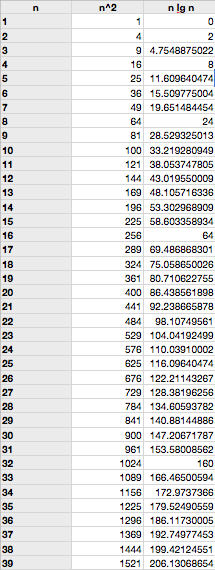
\includegraphics[width=80mm]{images/ss}
	\end{center}

\caption{Naive vs Recursive Max Subarray Search comparison}
\label{find_arr_compare}
\end{figure}

\begin{figure}[!h]

	\begin{center}
	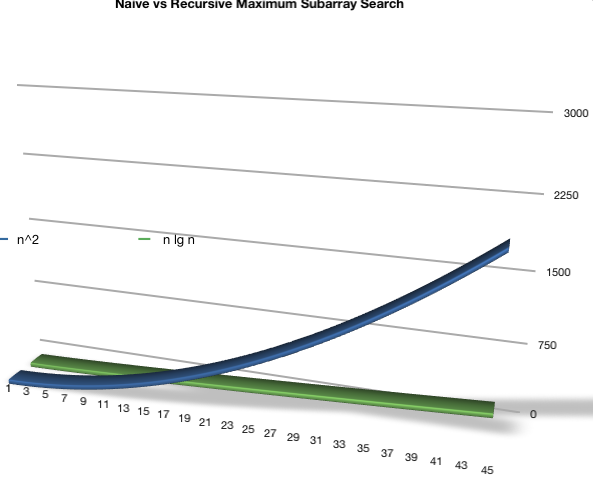
\includegraphics[width=120mm]{images/ss_graph}
	\end{center}

\caption{Naive vs Recursive Max Subarray Search comparison graph}
\label{find_arr_compare_graph}
\end{figure}

\end{document}